\documentclass[mathserif]{beamer}
%\documentclass[8pt,handout, ignorenonframetext]{beamer}
%\documentclass[handout,9pt]{beamer}
%\usepackage{pgfpages}
%\pgfpagesuselayout{2 on 1}[a4paper,border shrink=5mm]
\usetheme{Madrid}
\usecolortheme{beaver}
\beamertemplatenavigationsymbolsempty
\title{Visuals to Selected Resume Projects}
\author{}
\mode<presentation>
\institute{
}
\date{July 14, 2017}
\author[Gurgen Hayrapetyan]{
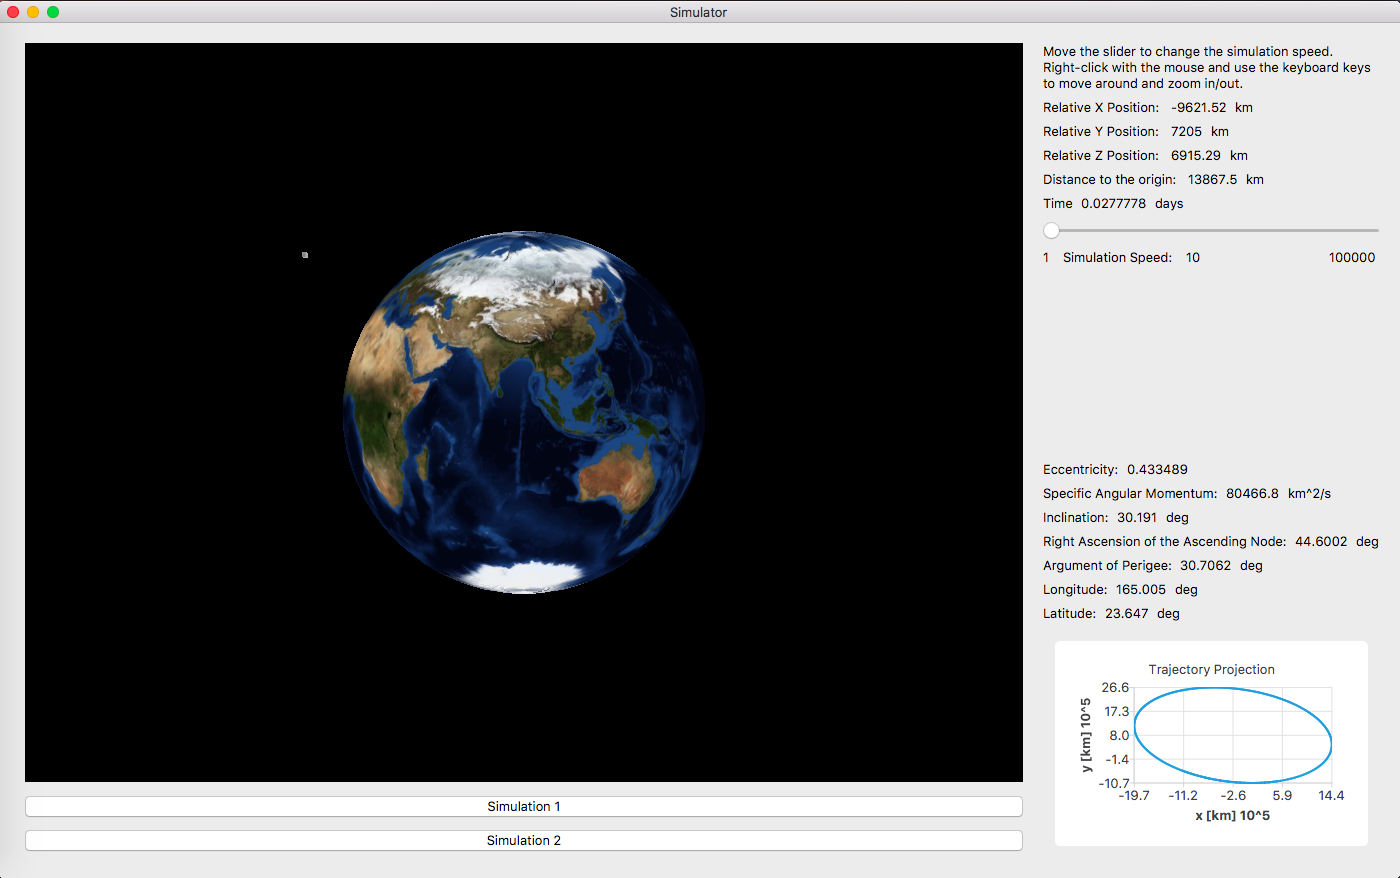
\includegraphics[height=3cm]{sat3.png}\\
Gurgen (Greg) Hayrapetyan}

\usepackage{mathrsfs}
\usepackage{amsmath}    % need for subequations
\usepackage{graphicx}   % need for figures
\usepackage{verbatim}   % useful for program listings
\usepackage{color}      % use if color is used in text
\usepackage{subfigure}  % use for side-by-side figures
\usepackage{amssymb}
\usepackage{multimedia}
\usepackage{hyperref}
\usepackage{wrapfig}

%\usepackage{media9} 

\usepackage{latexsym,amsmath,amsfonts,amscd}
\usepackage{amsmath}
\usepackage{amssymb}
\usepackage{graphicx}
\usepackage{yfonts}
\usepackage{color}
%\usepackage{showkeys}
\def\Put(#1,#2)#3{\leavevmode\makebox(0,0){\put(#1,#2){#3}}}

\renewcommand{\theequation}{\thesection.\arabic{equation}}

\newenvironment{frcseries}{\fontfamily{frc}\selectfont}{}
\newcommand{\textfrc}[1]{{\frcseries#1}}
\newcommand{\mathfrc}[1]{\text{\textfrc{#1}}}
%\newcommand{\cl}{\mathfrc{l}}
\newcommand{\cl}{\ell}

\def\beq{\begin{equation}}
\def\eeq{\end{equation}}
\def\beqa{\begin{eqnarray}}
\def\eeqa{\end{eqnarray}}
\def\eps{\varepsilon}

%\useoutertheme[subsection=false]{smoothbars}
\setbeamertemplate{footline}[text line]{} % makes the footer EMPTY


\begin{document}


\begin{frame}
\titlepage
\end{frame}

\begin{frame}
\frametitle{Computer Vision}

\begin{columns}[c]
\column{1.5in}
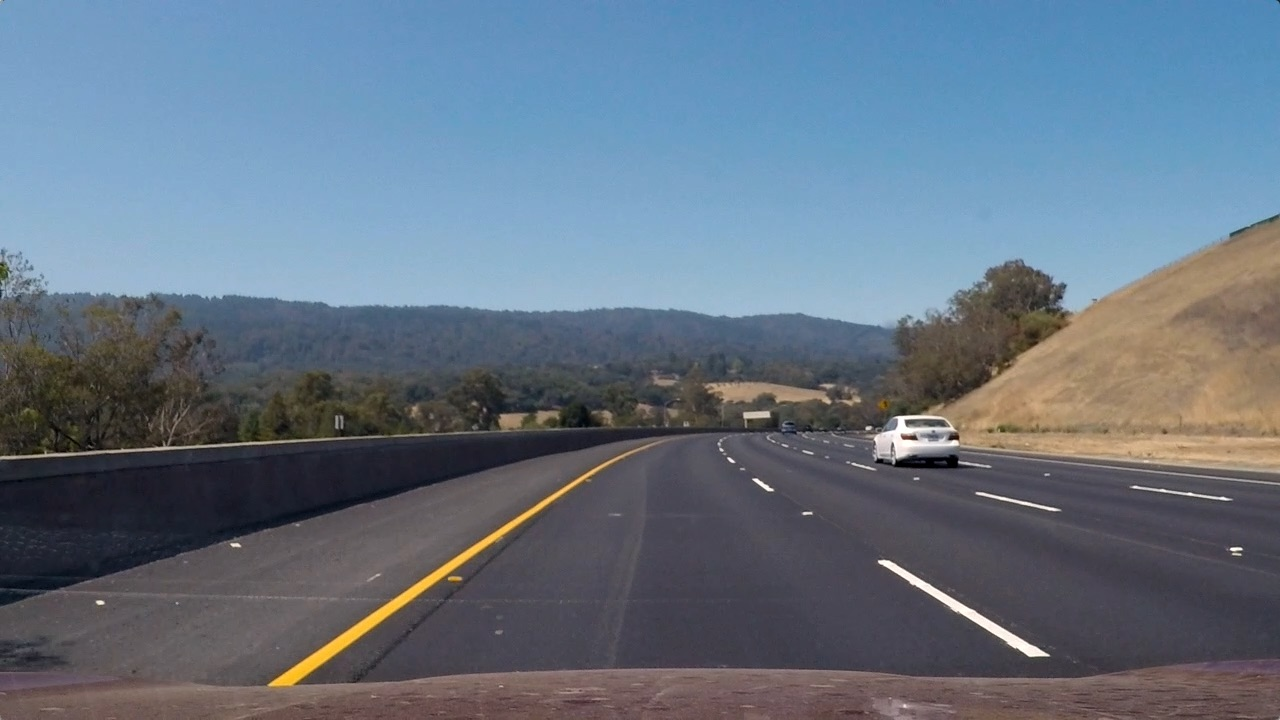
\includegraphics[width=45mm]{alf1.jpg}

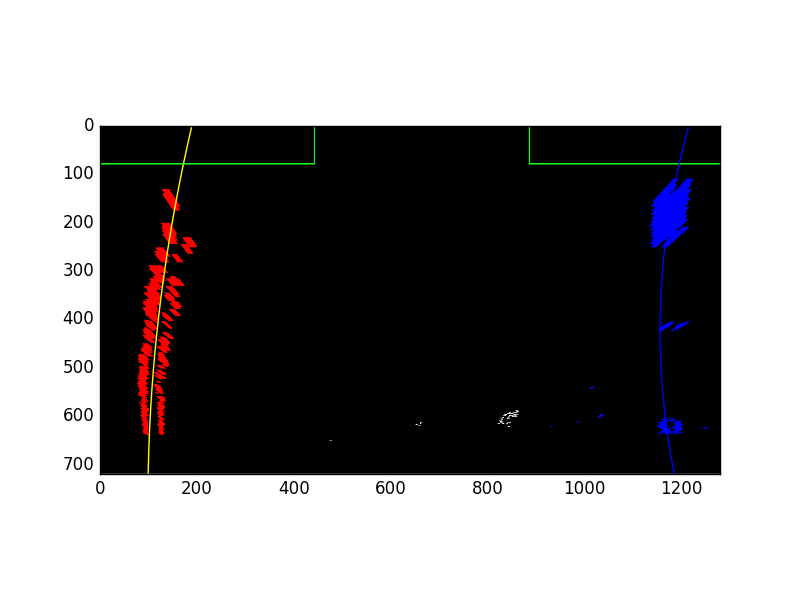
\includegraphics[width=5.5cm]{alf3.png}

\column{3in}
\begin{center}
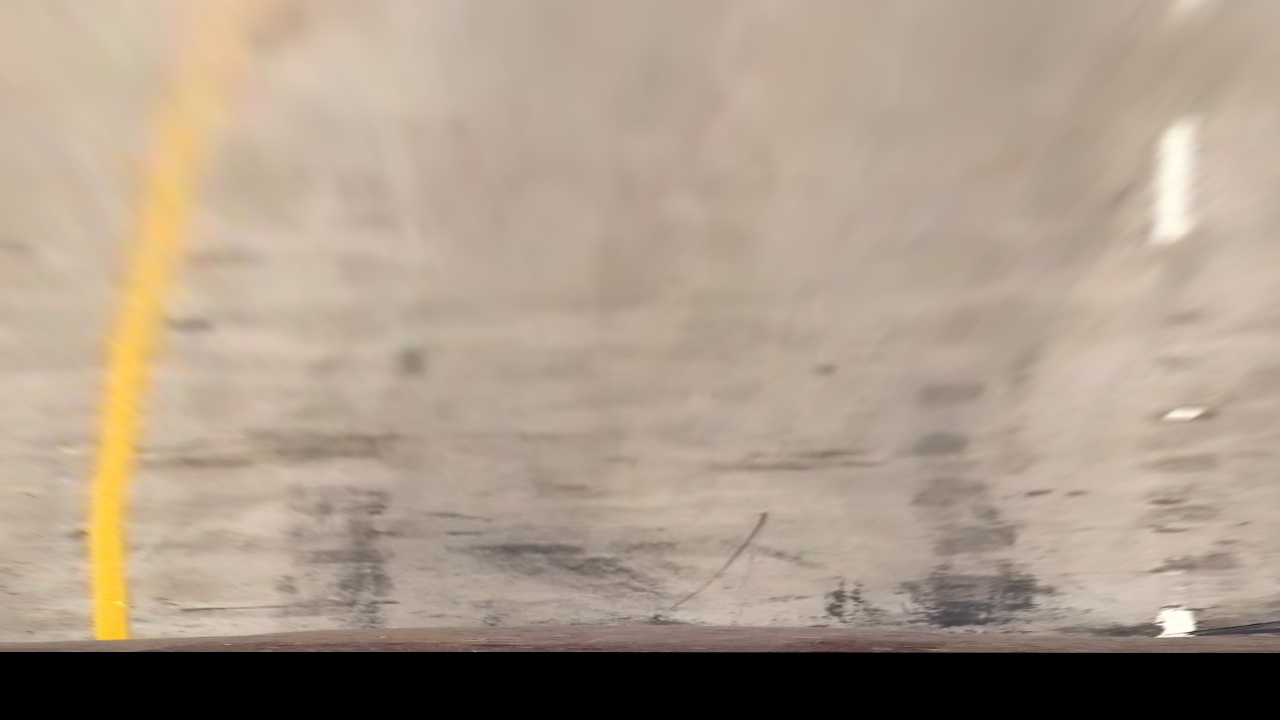
\includegraphics[width=5.5cm]{alf2.jpg}

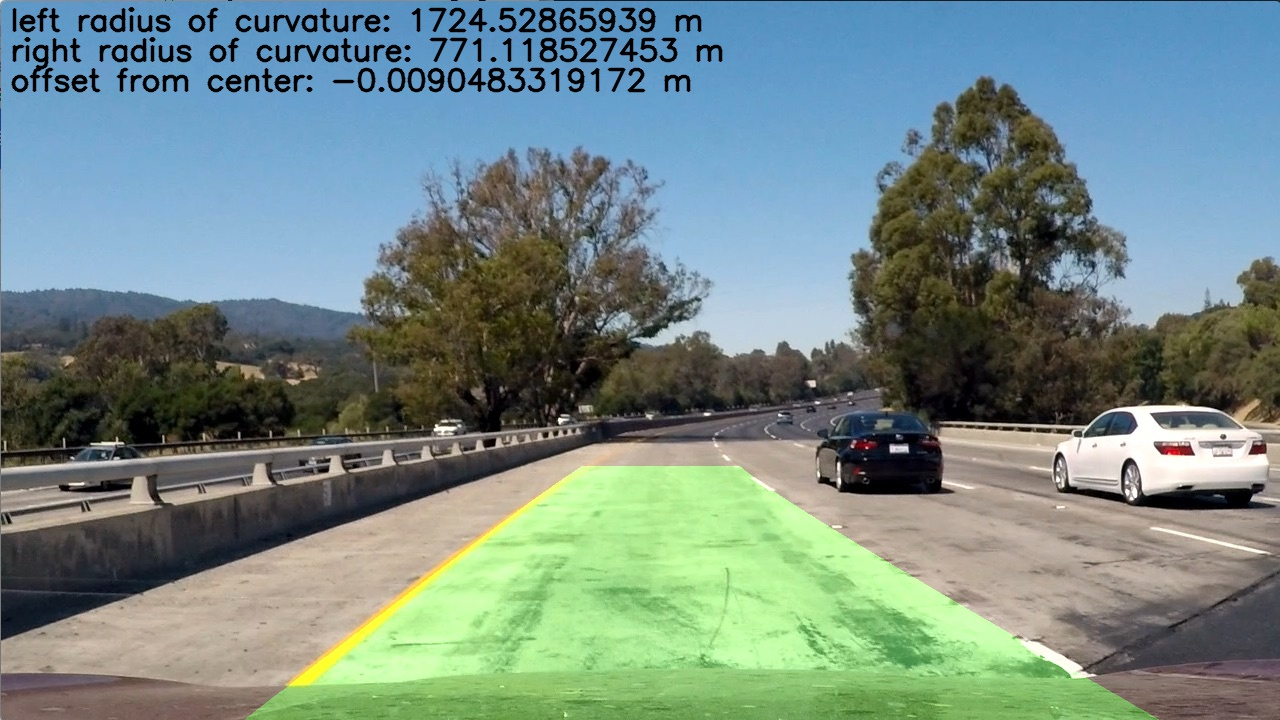
\includegraphics[width=5.5cm]{alf4.jpg}

\vspace{0.1cm}
\begin{columns}[c]
\column{1.5in}

\end{columns}
\end{center}
\end{columns}

\end{frame}

\begin{frame}
\frametitle{Vehicle Detection - Computer Vision and Machine Learning to Identify Vehicles}

\begin{columns}[c]
\column{1.5in}
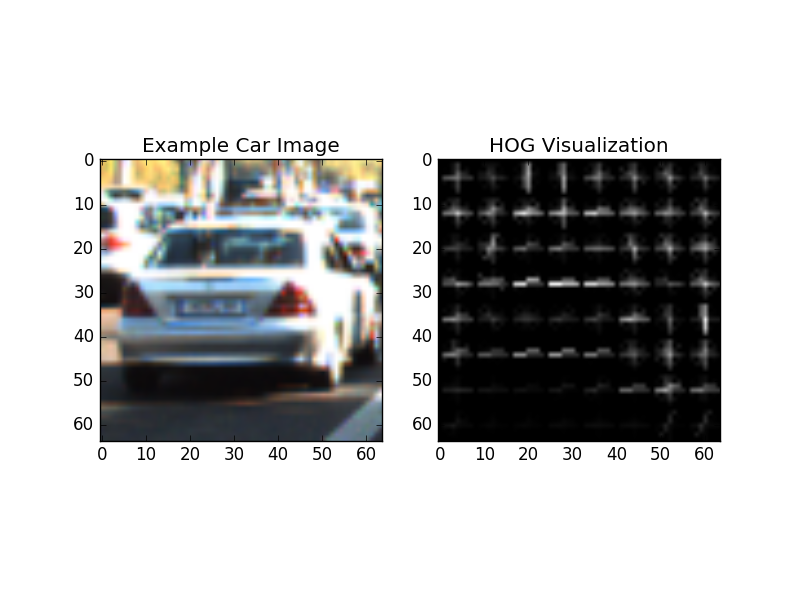
\includegraphics[width=45mm]{vd1.png}

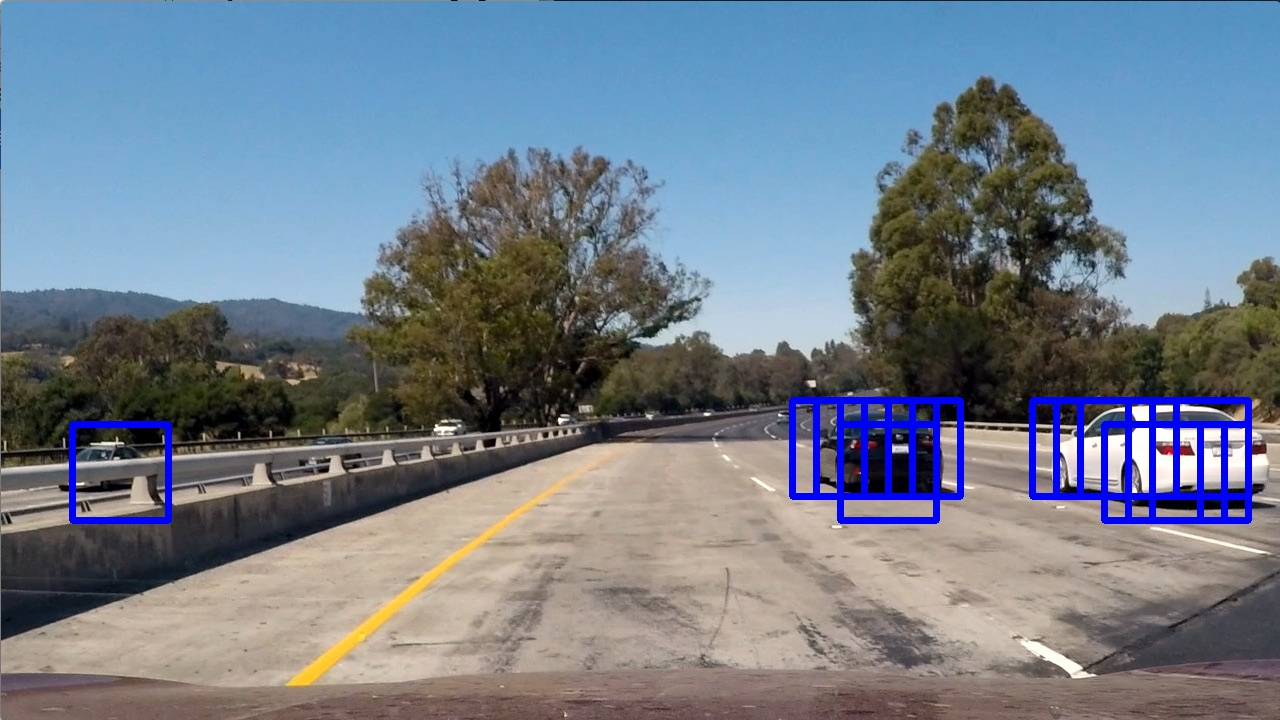
\includegraphics[width=5.5cm]{vd2.jpg}

\column{3in}
\begin{center}
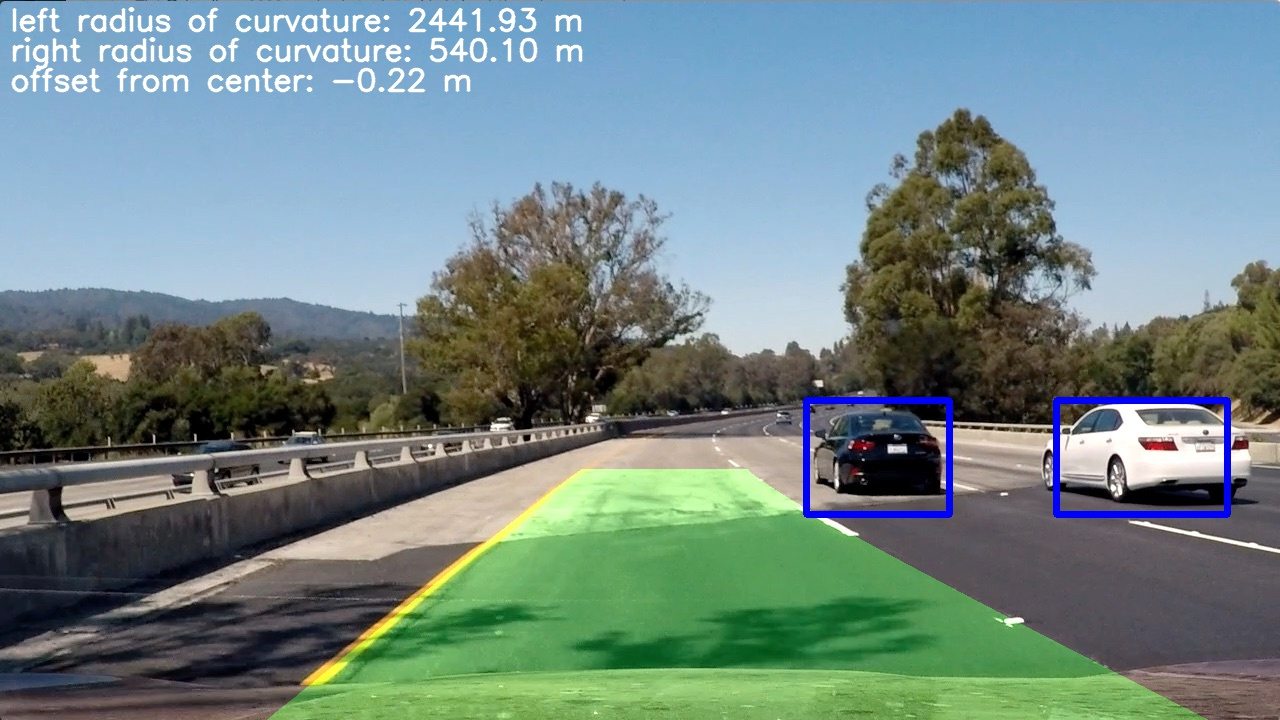
\includegraphics[width=7cm]{vd3.jpg}

\vspace{0.1cm}
\begin{columns}[c]
\column{1.5in}

\end{columns}
\end{center}
\end{columns}

\end{frame}
\begin{frame}
\frametitle{Adaptive Cruise Control Simulation}

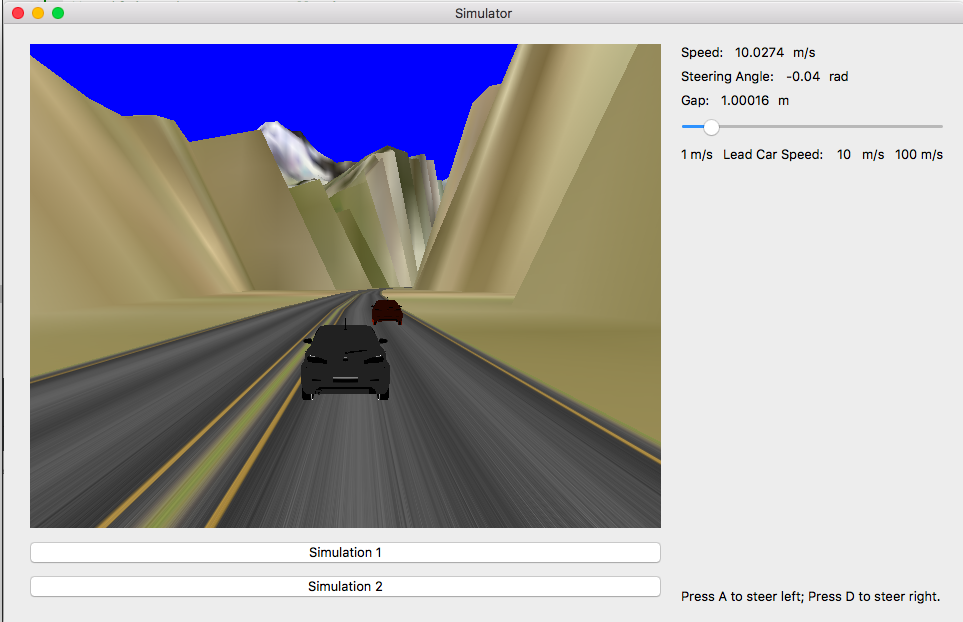
\includegraphics[width=4.7in]{SimulatorScreenShot.png}


\end{frame}

\begin{frame}
\frametitle{Restricted Three-Body Problem Simulation}

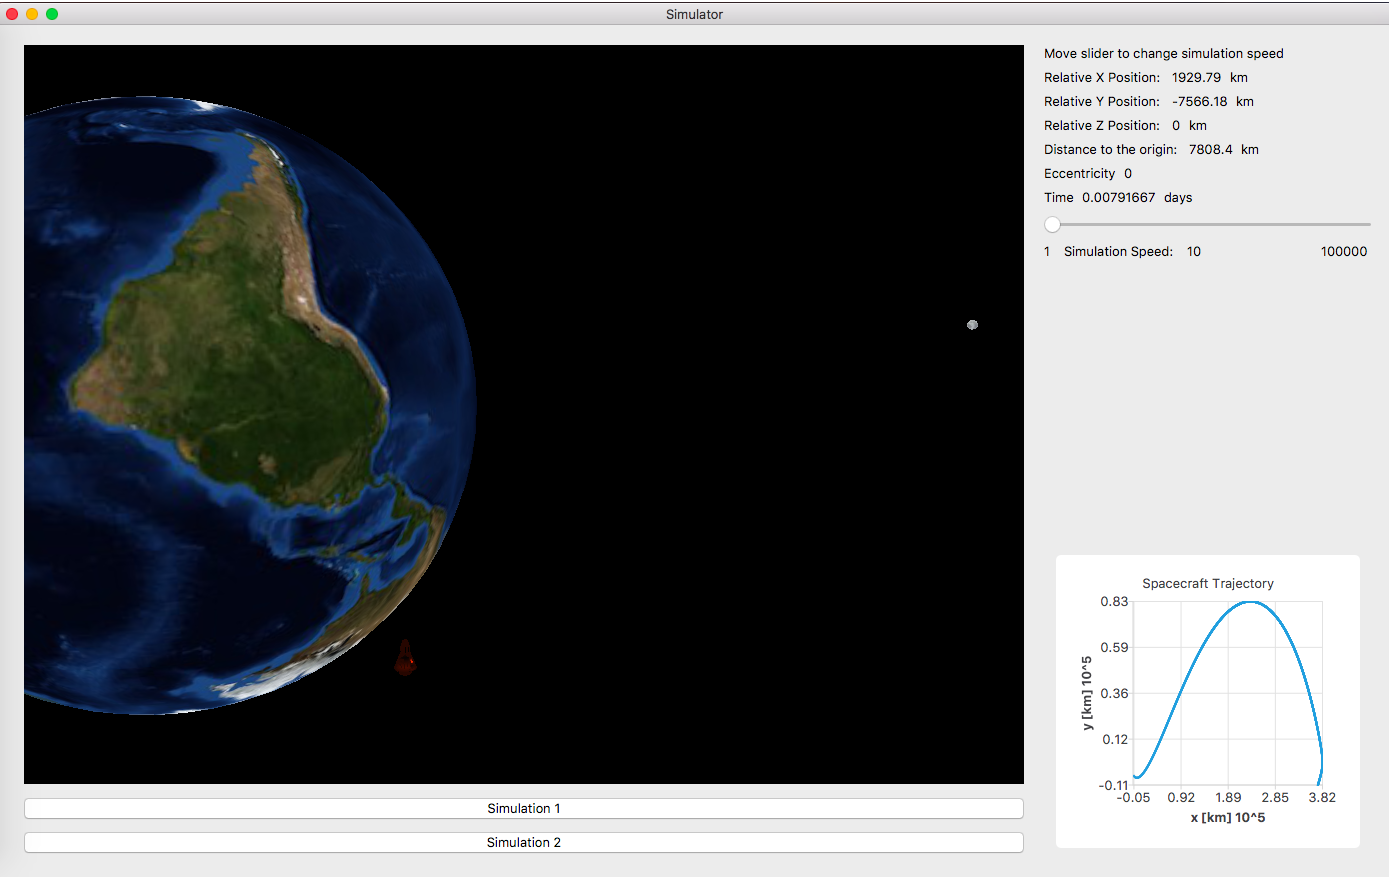
\includegraphics[width=4.7in]{Restricted3Body.png}


\end{frame}



\begin{frame}
\frametitle{Deterministic Satellite Tracking}

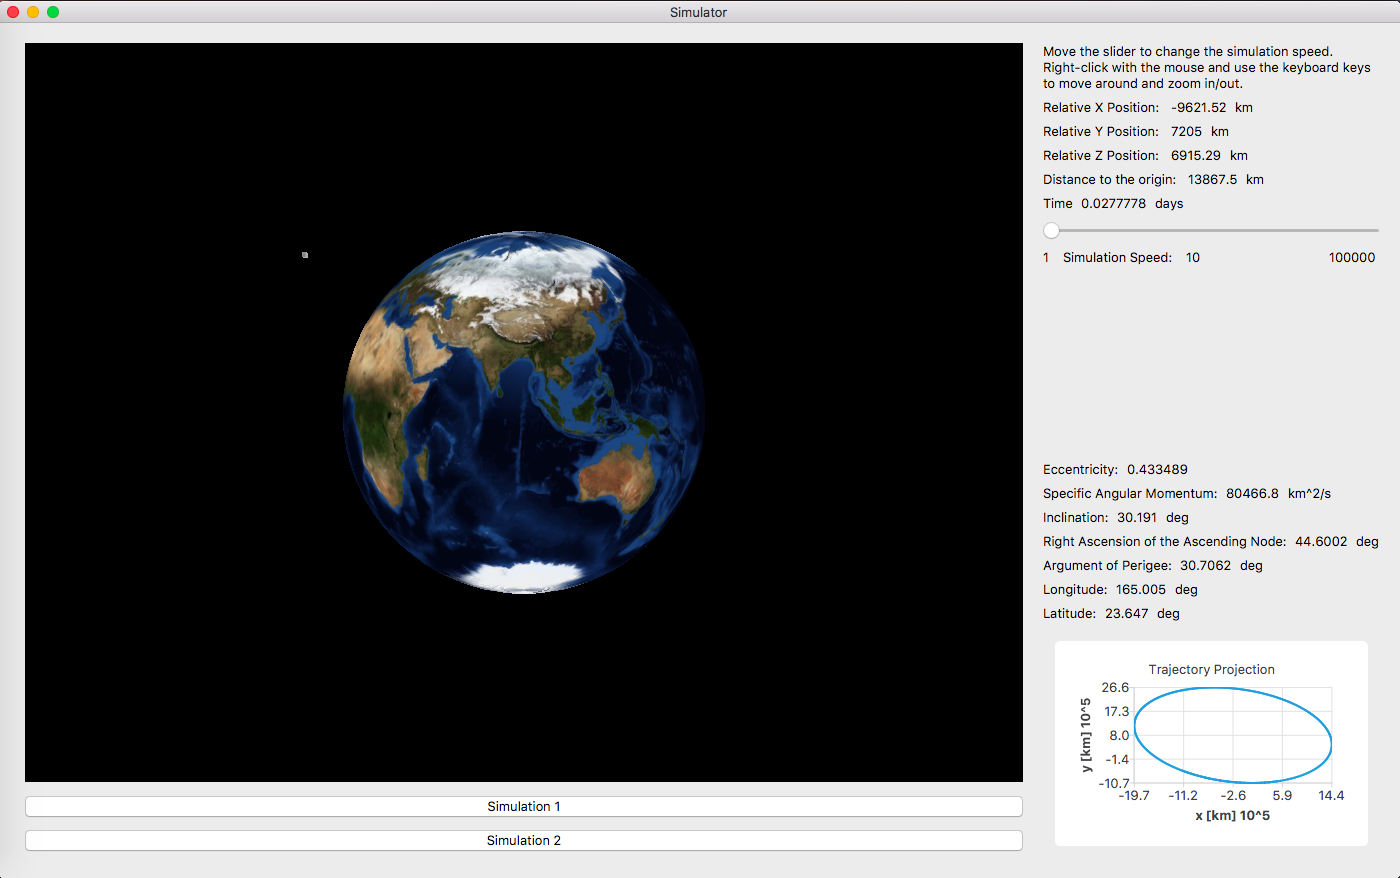
\includegraphics[width=3.5in]{sat3.png}

\begin{itemize}
\item Gibbs method
\item Lambert's problem
\end{itemize}

\end{frame}

\begin{frame}
\frametitle{Statistical Orbit Determination}

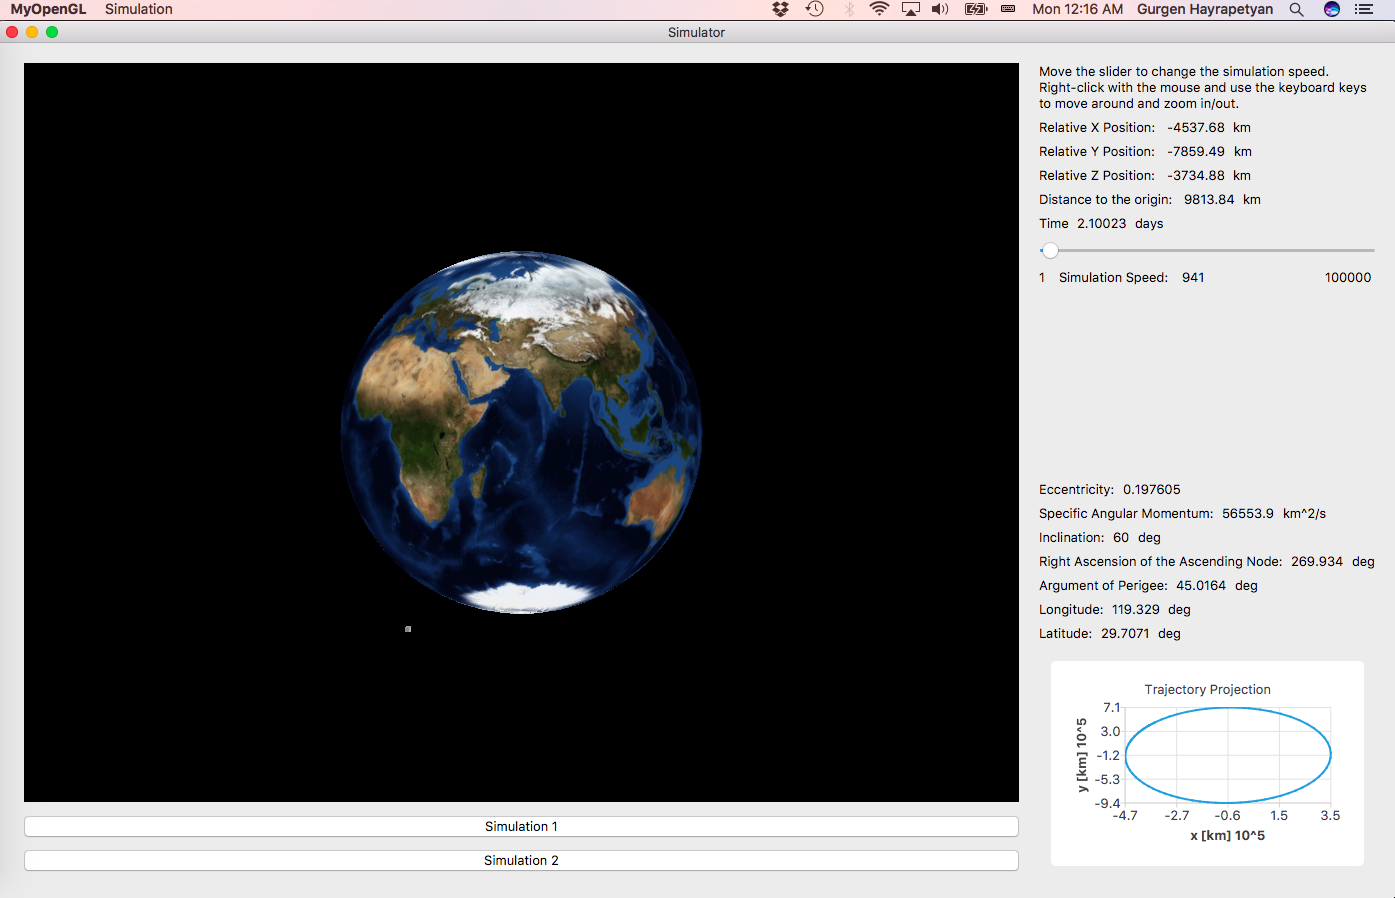
\includegraphics[width=3.5in]{sat2.png}

Active Work:

\begin{itemize}
\item Nonlinear system two point boundary value problem solver implementations in C++.
\item Optimal control codes for orbital maneuvers.
\end{itemize}

\end{frame}

\begin{frame}
\frametitle{Related Theoretical Work - Invariant Manifold Theory}

\begin{itemize}
\item Spectra of Functionalized Operators Arising from Hypersurfaces, ZAMP, (2014),
(coauthors: Keith Promislow).

\item Nonlinear Stability of Functionalized Flow  (coauthors: Keith Promislow), expected. 2017.

\item Main ideas:  Understanding full nonlinear evolution in the state space given linearized motion near equilibrium structures.

%\item These ideas were pioneered in the orbital mechanics context by Martin Lo and the team at JPL to calculate paths near Lagrange points.
\end{itemize}

%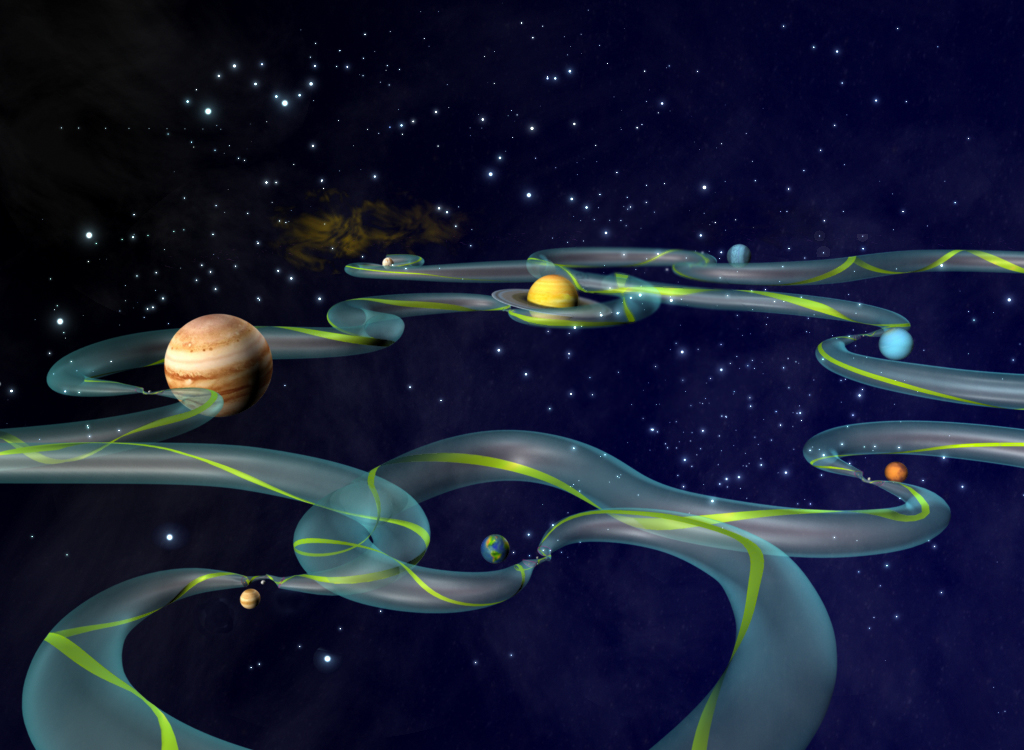
\includegraphics[height=1.5in, width=4.5in]{ish.jpg}

%\tiny{Source: From http://www.jpl.nasa.gov/releases/2002/release\_2002\_147.html}

\end{frame}

\begin{frame}
\frametitle{Aerodynamics - Python Code for Calculating Lift and Drag Coefficients for Airfoil using Thwaites' Method and Comparison to XFLR}


\begin{columns}[c]
\column{1.5in}
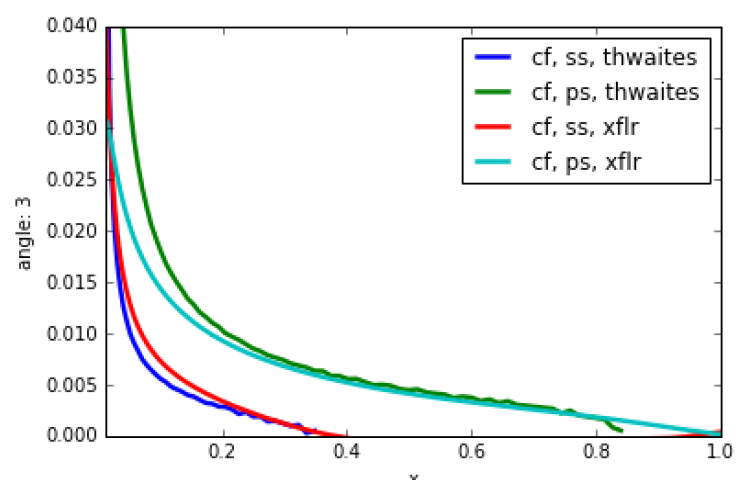
\includegraphics[width=45mm]{fd1.png}

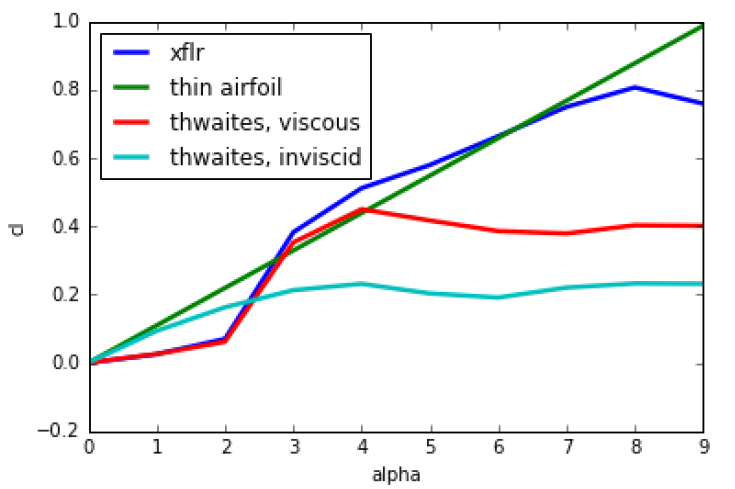
\includegraphics[width=5.5cm]{fd2.png}

\column{3in}
\begin{center}
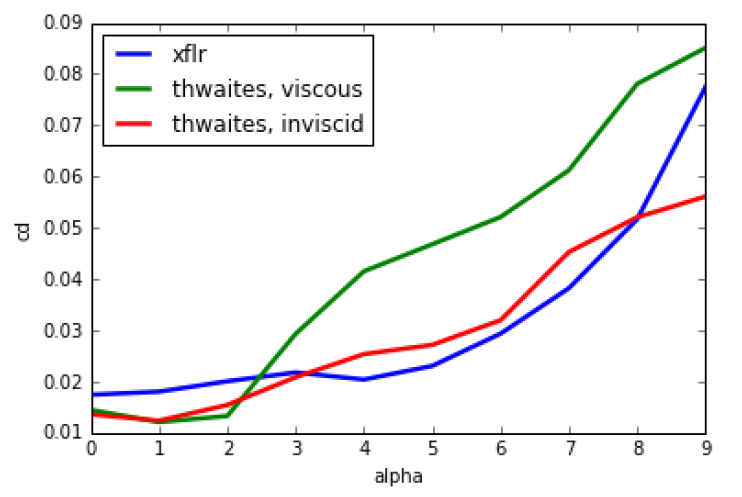
\includegraphics[width=7cm]{fd3.png}

\vspace{0.1cm}
\begin{columns}[c]
\column{1.5in}

\end{columns}
\end{center}
\end{columns}


\end{frame}

\begin{frame}
\frametitle{Stochastic Tool - Uncertainty Quantification Software for Engineering Design and Analysis}

\begin{columns}[c]
\column{1.5in}
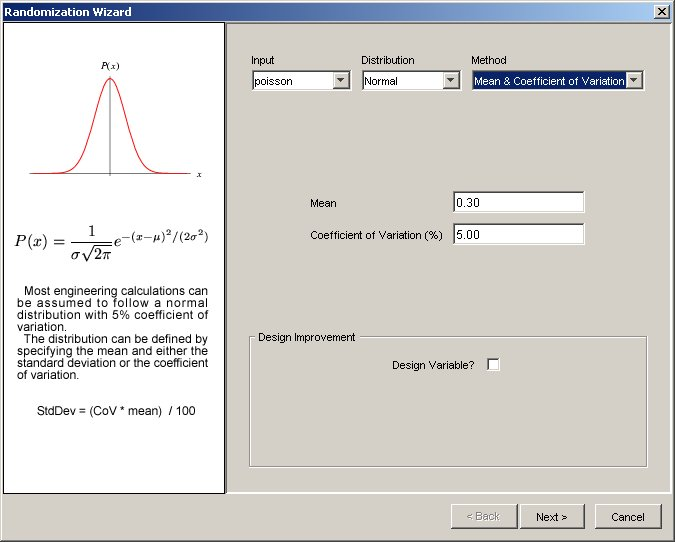
\includegraphics[width=45mm]{StocTool1.png}

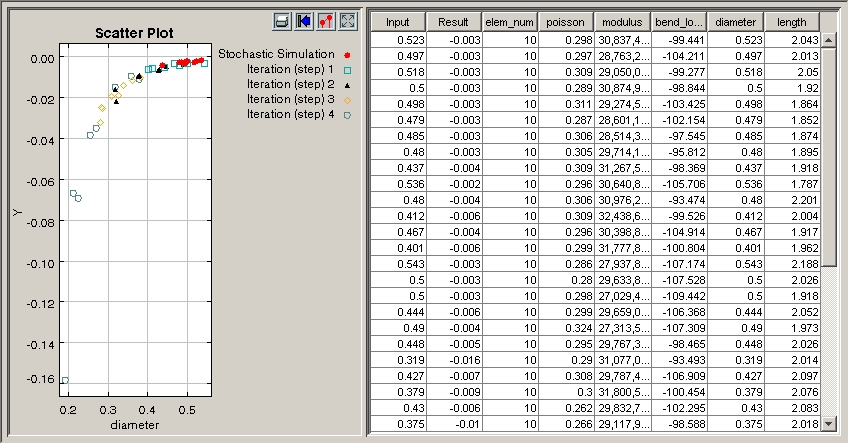
\includegraphics[width=5.5cm]{StocTool4.png}

\column{3in}
\begin{center}
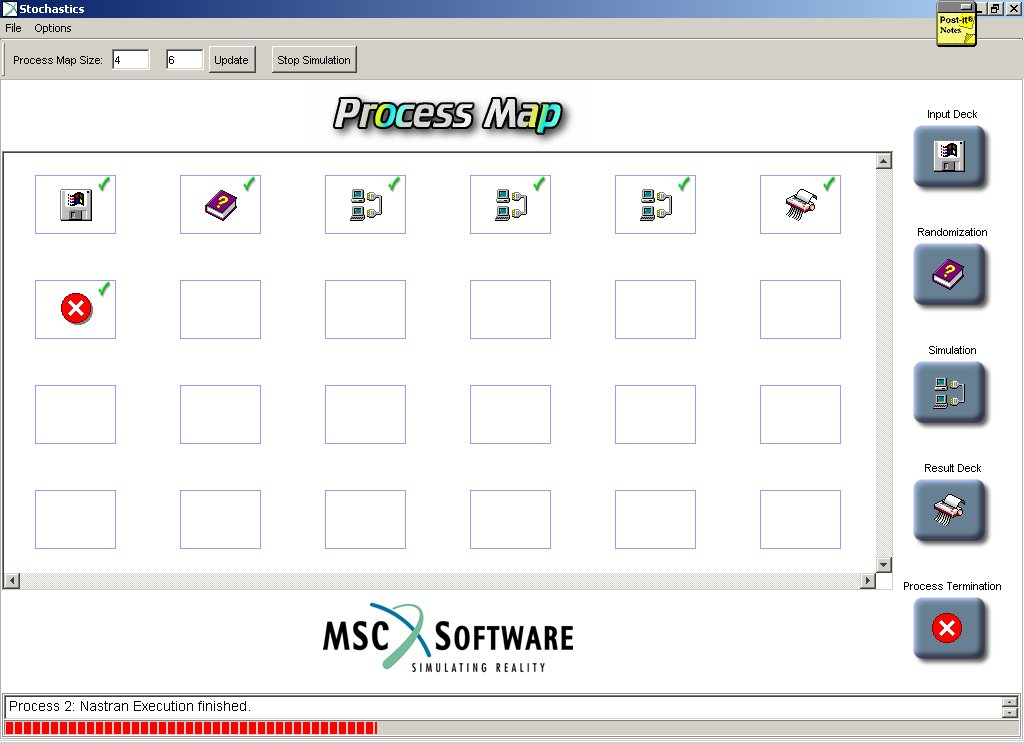
\includegraphics[width=7cm]{StocTool3.png}

\vspace{0.1cm}
\begin{columns}[c]
\column{1.5in}

\end{columns}
\end{center}
\end{columns}


\end{frame}

\end{document}



